%=======================02-713 LaTeX template, following the 15-210 template==================
%
% You don't need to use LaTeX or this template, but you must turn your homework in as
% a typeset PDF somehow.
%
% How to use:
%    1. Update your information in section "A" below
%    2. Write your answers in section "B" below. Precede answers for all 
%       parts of a question with the command "\question{n}{desc}" where n is
%       the question number and "desc" is a short, one-line description of 
%       the problem. There is no need to restate the problem.
%    3. If a question has multiple parts, precede the answer to part x with the
%       command "\part{x}".
%    4. If a problem asks you to design an algorithm, use the commands
%       \algorithm, \correctness, \runtime to precede your discussion of the 
%       description of the algorithm, its correctness, and its running time, respectively.
%    5. You can include graphics by using the command \includegraphics{FILENAME}
%
\documentclass[11pt]{article}
\usepackage{amsmath,amssymb,amsthm}
\usepackage{graphicx}
\usepackage[margin=1in]{geometry}
\usepackage{fancyhdr}
\usepackage{float}


\setlength{\parindent}{0pt}
\setlength{\parskip}{5pt plus 1pt}
\setlength{\headheight}{13.6pt}
\newcommand\question[2]{\vspace{.25in}\hrule\textbf{#1: #2}\vspace{.5em}\hrule\vspace{.10in}}
\renewcommand\part[1]{\vspace{.10in}\textbf{(#1)}}
\newcommand\algorithm{\vspace{.10in}\textbf{Algorithm: }}
\newcommand\correctness{\vspace{.10in}\textbf{Correctness: }}
\newcommand\runtime{\vspace{.10in}\textbf{Running time: }}
\pagestyle{fancyplain}
\lhead{\textbf{\NAME\ (\ANDREWID)}}
\chead{\textbf{HW\HWNUM}}
\rhead{\today}
\begin{document}\raggedright
%Section A==============Change the values below to match your information==================
\newcommand\NAME{Yao Xiao}  % your name
\newcommand\ANDREWID{2019180015}     % your andrew id
\newcommand\HWNUM{1}              % the homework number
%Section B==============Put your answers to the questions below here=======================

% no need to restate the problem --- the graders know which problem is which,
% but replacing "The First Problem" with a short phrase will help you remember
% which problem this is when you read over your homeworks to study.

\question{0}{Abstract}
End-to-end encryption is a method of secure communication that prevents third-parties from accessing data while it's transferred from one end system or device to another.
This article uses the E2EE-based Signal protocol to design a secure group chat, and implements a small message service based on E2EE encryption based on log security audits, enabling it to be used in secure encrypted communication applications.


\question{1}{Introduction} 

The signal protocol defines an encryption protocol for secure end-to-end encryption (E2EE). It was created by Open Whisper Systems for the secure messaging application TextSecure, but has since been released as an open source to the wider community. It has become very popular in consumer applications and has earned its name as the de facto standard for securing messaging and voice and video communications. Some of the biggest adopters include Google Allo, Facebook Messenger and WhatsApp, but more and more organizations use E2EE every day, because privacy, security and surveillance concerns are increasingly becoming the focus of public attention.

In short, E2EE allows us to ensure that our data is only visible to the intended recipient; even before sending via wire, the data will be encrypted on the client on the user's own device. This means that all the infrastructure in the middle (routing, messaging servers, databases, etc.) will never be able to see the data in its original format! This is very good-it means that we can completely eliminate the element of trust between the client and the server, so users do not have to worry about whether their data is really safe in the hands of the messaging provider. But more importantly, this means that any third party trying to intercept user communications in transit will definitely fail.

\subsection{Diffie–Hellman Key Exchange}

DH protocl allows the two parties to determine a "agreement key" in an insecure network without prior communication. This key can be used as a symmetric key in subsequent communications to encrypt message content. 
This avoids the risk of leakage caused by the agreement of keys between the two parties online. The principle of the DH protocol can be expressed by the following formula:

\begin{equation}
    DH(SK_A, PK_B) = Message Key\ S = DH(SK_B, PK_A)
\end{equation}

Both parties send their own public keys to each other, even if there is a hacker listening, he can only get the public key A, public key B, Alice uses her private key and Bob's public key to calculate the message key as S, Bob uses his private key and Alice's public key to calculate the message key is also S.\\
Both parties also determined the agreement key S, which can be used to derive the message key for encrypted communication. 
The hacker only knows theublic key A and the public key B, because he does not know the private key of either party, the key S cannot be calculated.

\begin{figure}[H]
    \centering
    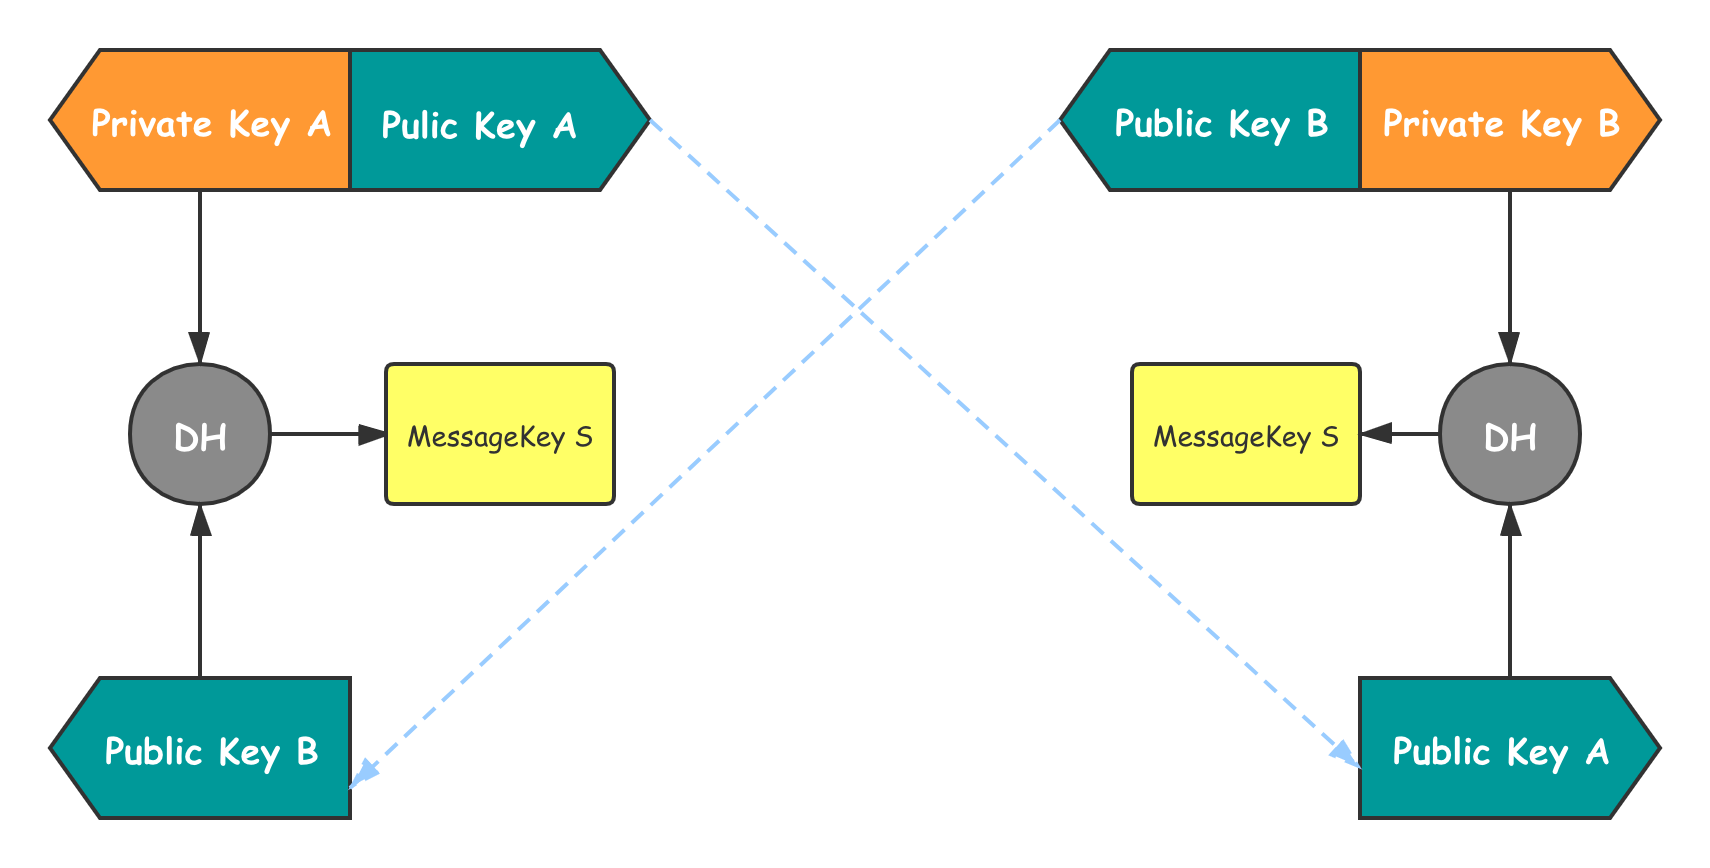
\includegraphics[width=1\textwidth]{Fig1}
    \caption{DH Protocol Flow}
\end{figure}

\subsection{X3DH}
The signal protocol uses the X3DH protocol to create the message key. X3DH protocol is based on DH protocol.\\
Alice and Bob each have a set of identity key pairs, with public keys published to central server:

\begin{itemize}
    \item Identity Key Pair --- A long-term Curve25519 key pair, creating during user registration and bound to user identity 
    \item Signed Pre Key --- A mid-term Curve25519 key, creating during user registration, signed by the identity key, and periodically rotated, this key may be to protect the identity key from being leaked
    \item One-Time Pre Keys --- One-time use Curve25519 key pair queue, generated during installation, supplemented when insufficient
\end{itemize}

Alice initiates session with Bob by generating an ephemeral key pair $EPK_A$ and calculating:
\begin{itemize}
    \item $DH_1 = DH(IPK_A, SPK_B)$
    \item $DH_2 = DH(EPK_A, IPK_B)$
    \item $DH_3 = DH(EPK_A, SPK_B)$
    \item $DH_4 = DH(EPK_A, OPK_B)$
\end{itemize}

\begin{figure}[H]
    \centering
    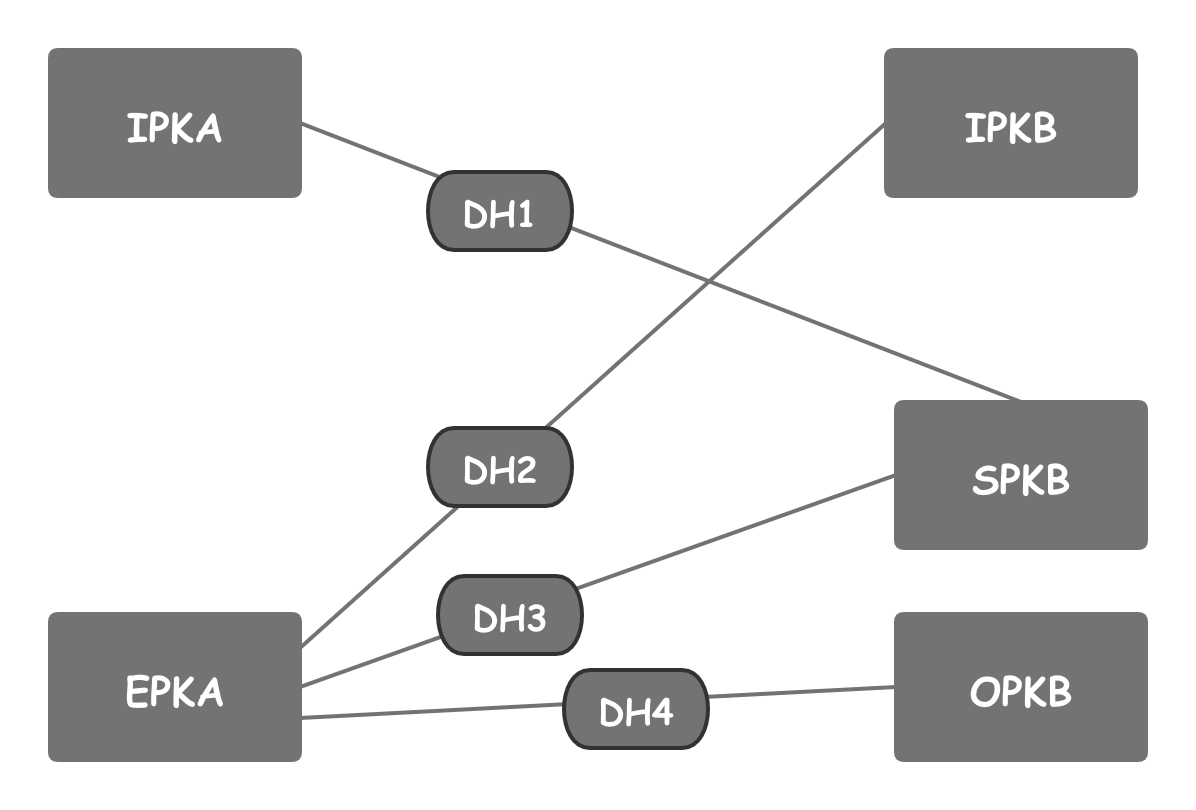
\includegraphics[width=0.8\textwidth]{Fig2}
    \caption{X3DH Flow}
\end{figure}

However, the DH key is too long to be used as a message key. The initial key needs to be KDF calculated to derive a fixed-length message key S:
\begin{equation}
    S = KDF(DH_1||DH_2||DH_3||DH_4)
\end{equation}

Alice uses the message key S to encrypt the message and sends it to Bob along with her identity public key IPK-A and temporary public key EPK-A. 
After receiving Alice's information, Bob takes out Alice's two public keys, together with his own key, and uses the same algorithm as Alice to calculate the message key S.


\subsection{KDF Chains Ratchet}

KDF is a key derivation function. By appending some data, the original key is exported to a new key to improve the confidentiality of the original key. when new message key is needed, "symmetric ratchet" is used.\\
The KDF algorithm can be used to store user passwords more securely. A common password management method is to store the hash value of the user password on the server to prevent hackers from obtaining the original user password after the server is attacked. It is safe to add other information to the user hash.\\
The server only saves the final key. 
The advantage of this password management method is that no matter how simple the password set by the user, the key stored by the server is very random and is difficult to be collided.

\begin{figure}[H]
    \centering
    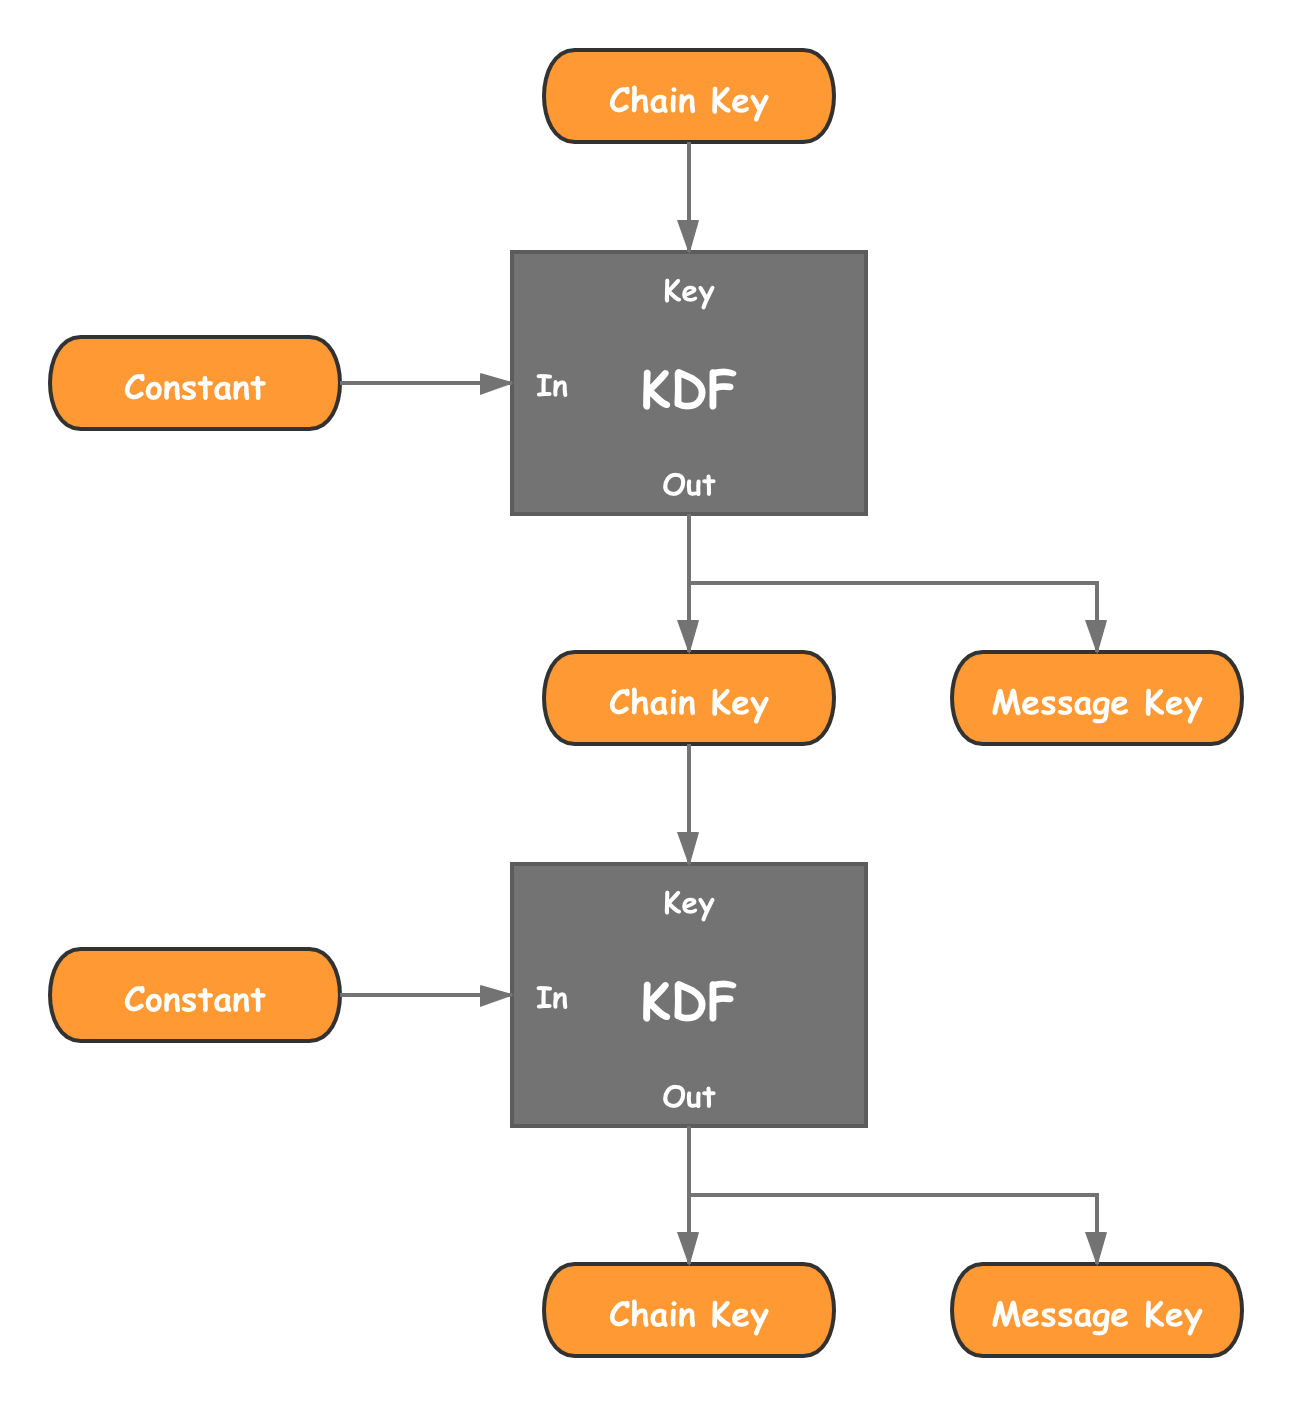
\includegraphics[width=0.8\textwidth]{Fig3} 
    \caption{KDF Chains Ratchet Flow}
\end{figure}


Use the KDF algorithm to derive a new key from the initial key. The new key is cut into two parts. The first half of the chain key is used as the input for KDF calculation, and the second half is used as the message key. 
Each iteration will generate a new message key.

Assuming that each message is sent in a ratchet step, the key of each message will be different, and because of the unidirectionality of the KDF algorithm, the key of this message cannot be pushed back to the previous message key. 
This ensures the forward security of the key.

However, this design cannot guarantee backward security. Once a hacker has cracked a certain key and mastered the content of the constant, then it can calculate all future message keys according to this algorithm.

Therefore, in order to ensure backward security, it is necessary to design an algorithm so that the constant introduced at each iteration is random, so as to ensure that the key of each message cannot be calculated backward. 
Signal Protocol ensures the randomness of constant by adding DH ratchet.

\subsection{DH Ratchet}
\label{dualsection}
The DH ratchet algorithm can ensure the randomness of the constant introduced in each calculation. As can be seen from the foregoing, the two key pairs can generate a secure negotiation key through the DH protocol. If one of the key pairs is replaced, the new negotiation key will also change. The DH ratchet algorithm is to replace a key pair in turn, and generate a different negotiation key each time, as the constant of the KDF ratchet algorithm. Each time a message cycle occurs, the DH ratchet updates the temporary key pair, the constant is updated, and the message key generated by the KDF ratchet algorithm has backward security.

According to the X3DH protocol, Alice wants to create a temporary key pair (EK-A), which is used to create the initial message key S. In fact, this temporary key pair has another purpose, which is to generate the first constant.

\begin{figure}[H]
    \centering
    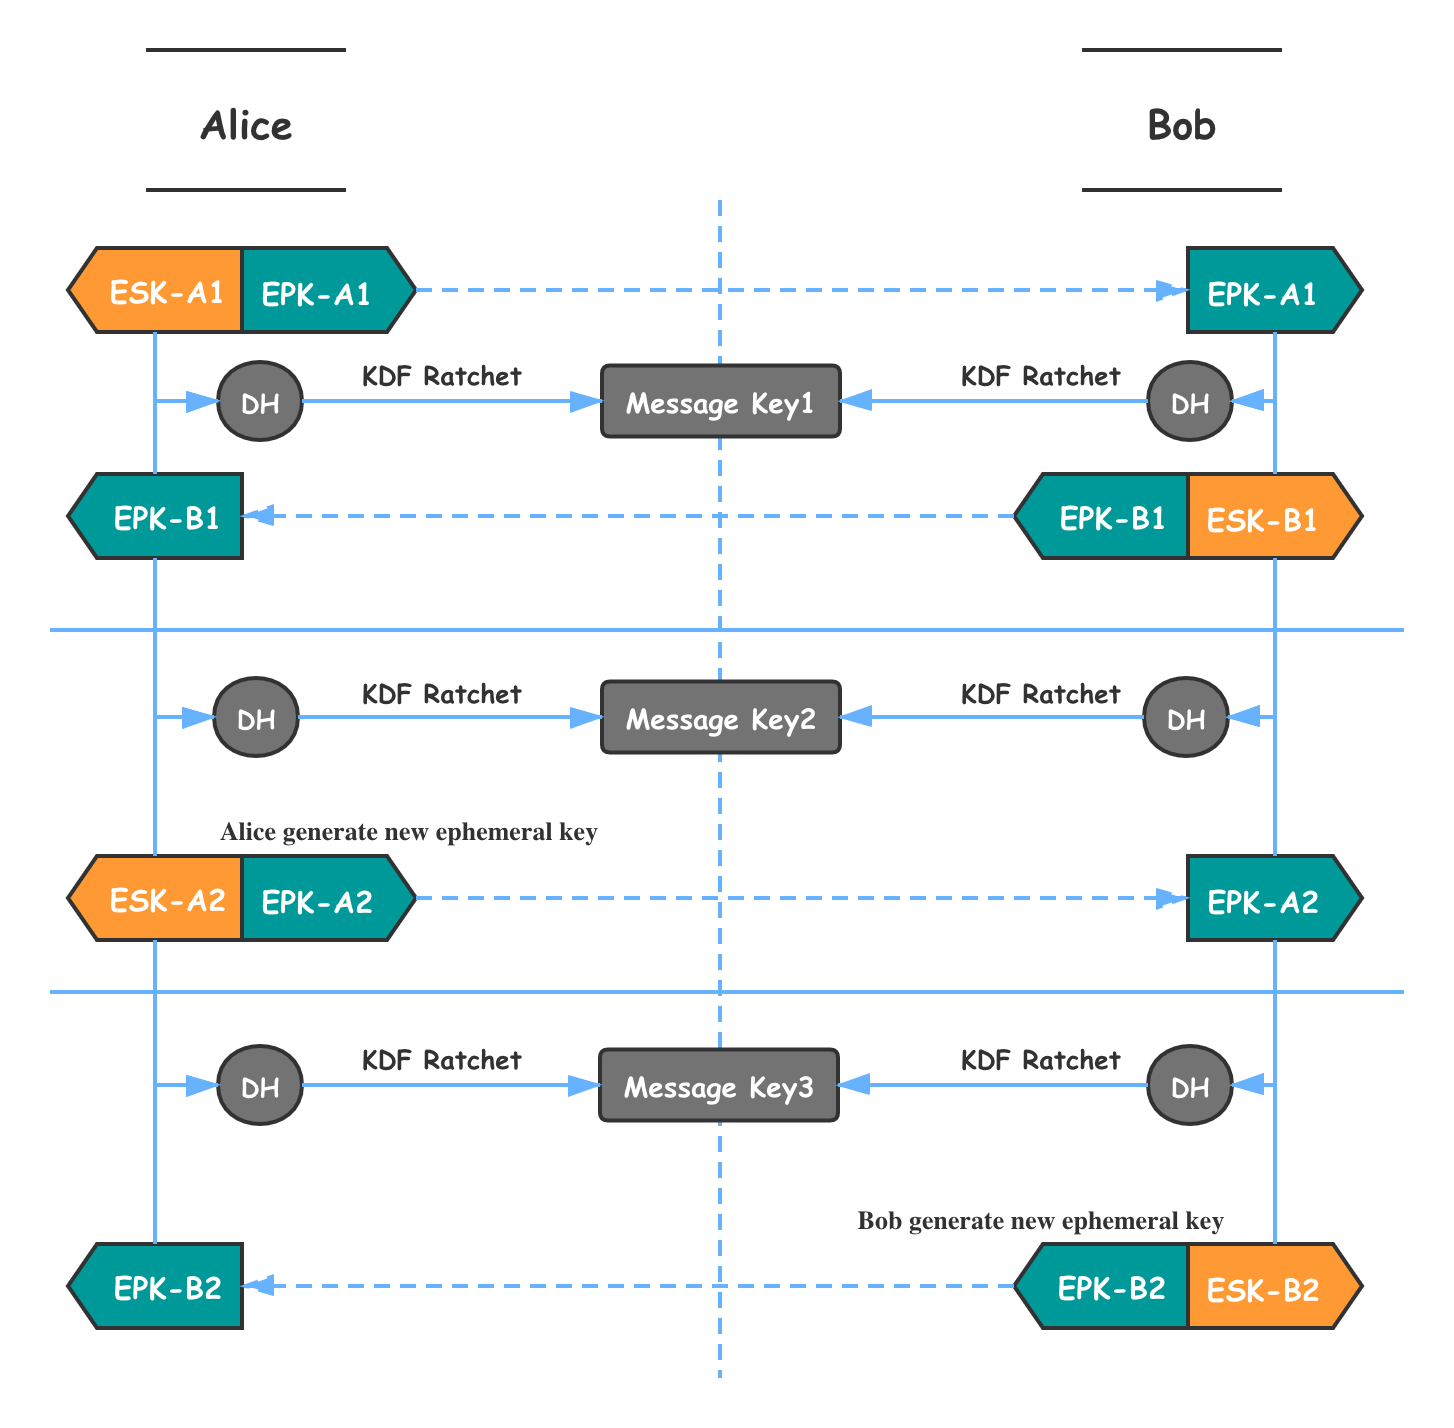
\includegraphics[width=0.8\textwidth]{Fig4}
    \caption{Double Ratchet Flow}
\end{figure}

As can be seen from the above figure, whenever you receive a message from the other party and respond, you must generate a new random DH key pair to generate a new DH key as a new salt. 
This ensures that the message key generated each time is completely random.

The method of double ratchet algorithm to deal with message loss or out of order is the DH key pair is not updated, which means that the salt introduced by the KDF ratchet remains unchanged, but the message key is still changed. 
The process is as follows:

\begin{figure}[H]
    \centering
    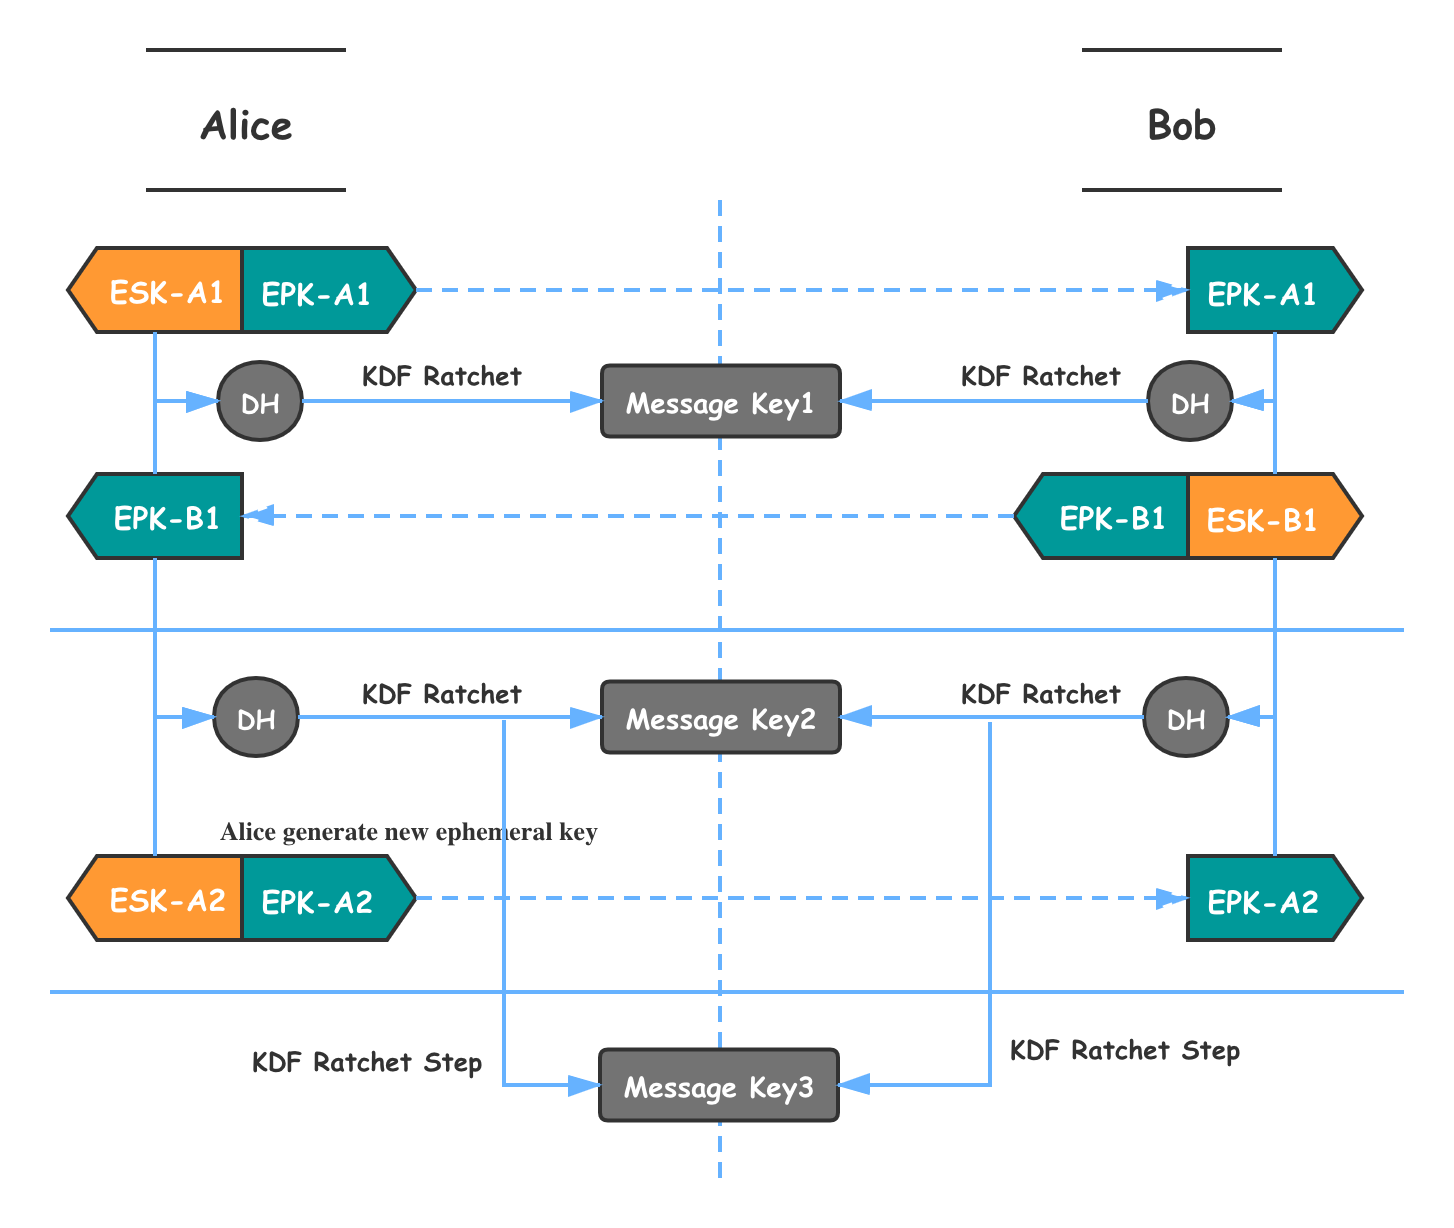
\includegraphics[width=0.8\textwidth]{Fig5} 
    \caption{Out-of-order Messages}
\end{figure}



\question{2}{Solution related to issue 1}

From the above introduction, it can know several types of keys that may be used.

\textbf{Public key type:} Identity Key Pair | Signed Pre Key | One-Time Pre Keys


\textbf{Session key type:}
\begin{itemize}
    \item Chain Key --- 32-byte value, used to create the message key
    \item Message Key --- 80-byte value, used to encrypt the message content. 
    32 bytes are used for AES-256 key, 32 bytes are used for HMAC-SHA256 key, and 16 bytes are used for IV.
\end{itemize}


\subsection{Group chatting}

\subsubsection{Register}
\label{section:register}

During registration, the client sends the identity public key, the signed pre-shared public key and a batch of one-time pre-shared public keys to the server. 
The server stores the public key related to the user's identity, and the server cannot access the private key of any client to ensure security.

\subsubsection{Exchange messages}
\label{section:em}
The message key is short-lived and changes every time the message is sent, so that the message key used to encrypt the message cannot be reconstructed from the session state after it has been sent or received.
Use the double ratchet algorithm mentioned in \ref{dualsection} to provide forward security

\subsubsection{Calculate the message key through the chain key}
\label{section:cm}
The calculation is as follows
\begin{equation}
    Message \ Key = HMAC-SHA256(Chain\ Key, 0\times 01)
\end{equation}
\begin{equation}
    Chain \ Key = HMAC-SHA256(Chain\ Key, 0\times 02)
\end{equation}
This forms a forward ratchet chain key, which also means that the stored message key cannot be used to derive the current or past chain key value.

\subsubsection{Transmission security}
All communication between the client and server is layered in a separate encrypted channel. 
On iOS and Android, these end-to-end encrypted clients can use Noise Pipes, using Curve25519, AES-GCM, and SHA256 in the Noise Protocol Framework to achieve long-term interactive connections.
\begin{itemize}
    \item Encrypt hidden metadata to prevent unauthorized network monitoring. 
    No information about the identity of connected users
    \item The client's security authentication information is not stored on the server. 
    The client uses the Curve25519 key for authentication, so the server only saves 3. The client public authentication key. 
    If the user database of the server is compromised, personal authentication 3. credentials will not be disclosed
\end{itemize}

\subsubsection{Group message}
\textbf{First: } (1) Each group member must first generate a random 32-byte KDF \textbf{\emph{Chain Key}}, which is used to generate a message key to ensure the forward security of the message key.
(2) Each group member must generates a random Curve25519 \emph{Signature Key} key pair for message signature. 
(3) Combines the 32-byte \textbf{\emph{Chain Key}} and the \textbf{\emph{Public Key}} from the \emph{Signature Key} into a \textbf{\emph{Sender Key}} message.
(4) Each group member encrypts and sends the \textbf{\emph{Sender Key}} to other members individually. 
At this time, each member has the \textbf{\emph{Chain Key}} and Signature \textbf{\emph{Public Key}} of all members in the group

\begin{figure}[H]
    \centering
    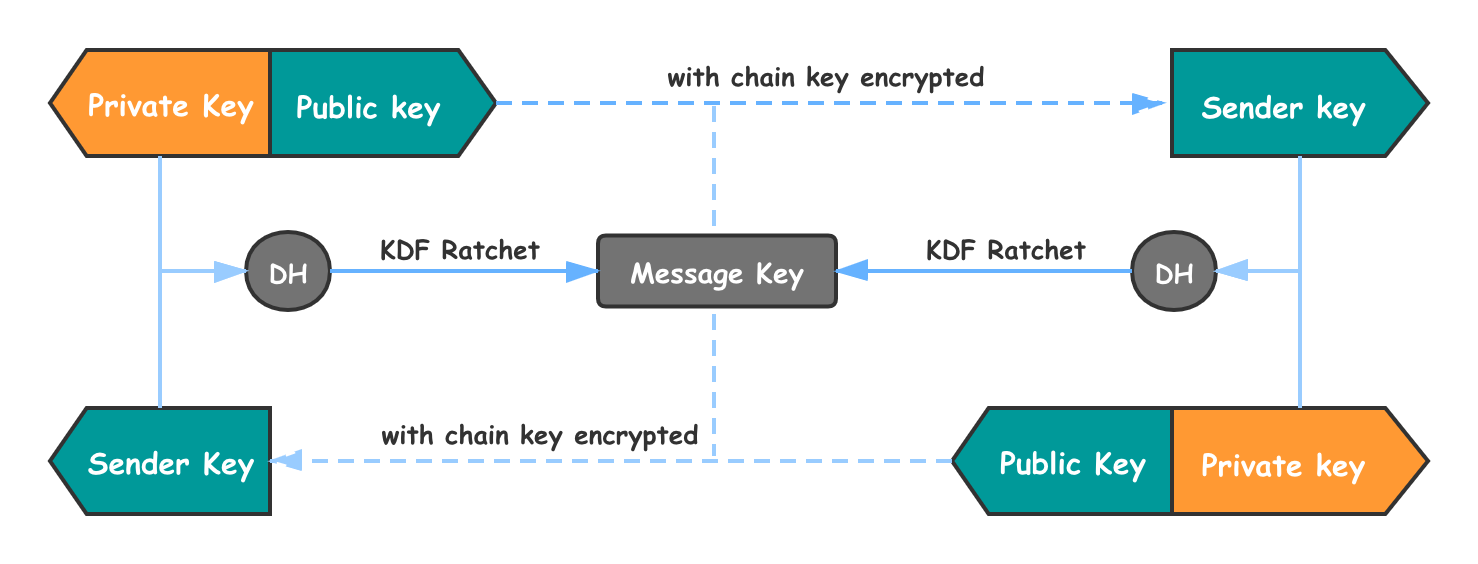
\includegraphics[width=0.8\textwidth]{Fig6}
    \caption{Sender Key}
\end{figure}
\textbf{Send and receive: } (1) When a member sends a message, first use the KDF chain ratchet algorithm to generate the \textbf{\emph{Message Key}}, and update \textbf{\emph{Chain Key}}.
(2) The sender encrypts the message using AES256 in CBC mode.
(3) The sender signs the ciphertext using the Signature \textbf{\emph{Private Key}}
(4) The sender sends a single cipher text message to the server, and the server distributes the message to all group members.
(5) After receiving the encrypted message, the other members first use the sender's Signature \textbf{\emph{Public Key}} to verify. After the verification is successful, the corresponding \textbf{\emph{Chain Key}} is used to generate the \textbf{\emph{Message Key}} and decrypt the message with the \textbf{\emph{Message Key}}.

\textbf{Exit: } When a group member leaves, all group members clear their \textbf{\emph{Sender Key}} and regenerate it, and send it to each member individually again. 
By doing this, the members who leave can't view the messages in the group.

From the above analysis, we can see that a person in different groups will generate different chain key and signature key pairs to ensure the isolation between the groups.


\subsubsection{Other solution}
This is the way to have a \textbf{\emph{Sender Key}}, each member has the chain key and signature public key of all members in the group.
Considering that there is no Sender Key.\\

Each group message is considered a direct message to the recipient. Therefore, if there are N participants, the signal client sends N messages and encrypts each participant's ratchet key separately. We need to have a separate ratchet state and separate session settings so that the ratchet state is inconsistent with that of personal messaging, which prevents the server from knowing which messages are sent for the group, and which is a direct message.

\question{3}{Solution related to issue 2}
The solution is the method of E2EE protocol plus log security audit. And The registration process is as shown \ref{section:register} and will not be repeated here.

\subsubsection{Session setup}
To communicate with another user, the client needs to establish an encrypted session. 
Once the encrypted session is created, the client does not need to create the session again unless the session fails, such as reinstalling the application or replacing the device.\\
(1) The session initiator applies for the recipient's Public Identity Key, Public Signed Pre Key, and One-Time Pre Key.
(2) The server returns the requested public key. 
One-Time Pre Key is used only once, so it will be deleted from the server after the request is completed. 
One-Time Pre Key is used up and has not been replenished, it returns empty.
(3) The initiator saves the recipient's Identity Key as \textbf{\emph{IRK}}, the signed Signed Pre Key as \textbf{\emph{SRK}}, and the One-Time Pre Key as \textbf{\emph{ORK}}.
(4) The initiator generates a temporary Curve25519 key pair as \textbf{\emph{EK}}.
(5) The initiator loads its own Identity Key as the \textbf{\emph{IDK}}.
(6) The initiator calculates the Master Key
\begin{equation}
\begin{split}
Master\ Key =& ECDH ( IDK, SRK) || ECDH(EK, IRK) || \\
    &ECDH ( EK, SRK)|| ECDH ( EK, ORK)
\end{split}
\end{equation}
If there is no One-Time Pre Key, the final ECDH will be ignored.\\
(7) The initiator uses the HKDF algorithm to create a Root Key and Chain Keys from Master Key.

\subsubsection{Receive session}
After establishing a long-term encrypted session, the initiator can immediately send a message to the recipient, even if the recipient handles the offline state. 
Before the receiver responds, all messages from the initiator will contain the information needed to create the session. 
This includes the sponsor's EK and IK.\\
(1) The recipient uses his own private key and the public key in the message header to calculate the corresponding master key.
(2) The recipient deletes the One-Time Pre Key used by the initiator.
(3) The initiator uses the HKDF algorithm to derive the corresponding Root Key and Chain Key from the master key.

\subsubsection{Exchange message and calculate message key}
See in \ref{section:em} and \ref{section:cm}

\subsubsection{Calculate chain key by root key}
Each message sent comes with a short-term Curve25519 public key. 
Once the response is received, the new Chain Key is calculated as follows. It should be noted that a chain key can only send messages to one user, so the message key cannot be reused.
\begin{equation}
    Ephemeral\ Key  = ECDH(EK-Sender, EK-Receiver)
\end{equation}

\begin{equation}
    Chain\ Key,\ Root\ Key =  HKDF(Root\ Key, Ephemeral\ Key)
\end{equation}


\subsection{Security Audi}

After completing the message service architecture, the audit function needs to be built. 
My idea is to use the log security audit method. The system log can record the encryption algorithm, whether the user's chat record is plain text, etc., and authorized users or third-party security agencies can view the system log to determine the security of the product.\\
Two concepts are introduced here: (1) Trusted Log Service Module(TLM), the verifier can verify the correctness of the behavior of the trusted log service through remote proof.
(2) Security Audit Module(SAM), recording security events running in the system and communicate with the trusted log service.


When the verifier needs to view the system log, he needs to communicate with the trusted log service module to obtain the required log information from the trusted log service module. 
Not only does TLM need to verify the integrity of the verifier, but also the verifier needs to verify the integrity of TLM. 
The verifier can be sure that the received logs have not been tampered with, and the verified party, TLM, is also authentic. 
The verifier obtains the clear text information of related log entries, but cannot obtain the clear text information of log entries in other log files.

The process of verifying the log is as follows:
\begin{enumerate}
    \item The verifier first needs to verify the integrity of the TLM operating environment and initiate a request to verify its integrity to the trusted server. 
    the trusted server collects the integrity information, and the platform where the TLM is located uses the signature key to sign the current constant, and sends the signed constant value and integrity metrics to the verifier
    \item The verifier verifies the integrity of the TLM operating environment, verifies the integrity of the integrity measurement log through the constant value, and ensures that the log file has not been tampered with; verifies the correctness and legality of the entries in the integrity measurement. 
    correctness and legality refer to the environment in which the platform on which TLM runs is free of malicious software. 
    if the verification is passed, continue the agreement, if the verification is not passed, then stop
    \item The verification sends a message to the TLM. the content of the message includes: the identity information of the verifier, the requested log entry, the message freshness identification, etc., and the request log information $L_j$
    \item TLM requests the information of log entry $L_j$ from SAM
    \item SAM sends the information of log entry $L_j$ to TLM
    \item TLM checks the access control information of log entry $L_j$ and checks whether the verifier meets the access control requirements. 
    based on its initial key $A_0$, generate the encryption key and authentication key $E_j$ of the log entry $L_j$, and send $E_j$ and $L_j$ to the verifier
    \item The log can only be decrypted when the verifier has access control secret information $W_j$
\end{enumerate}


\begin{figure}[H]
    \centering
    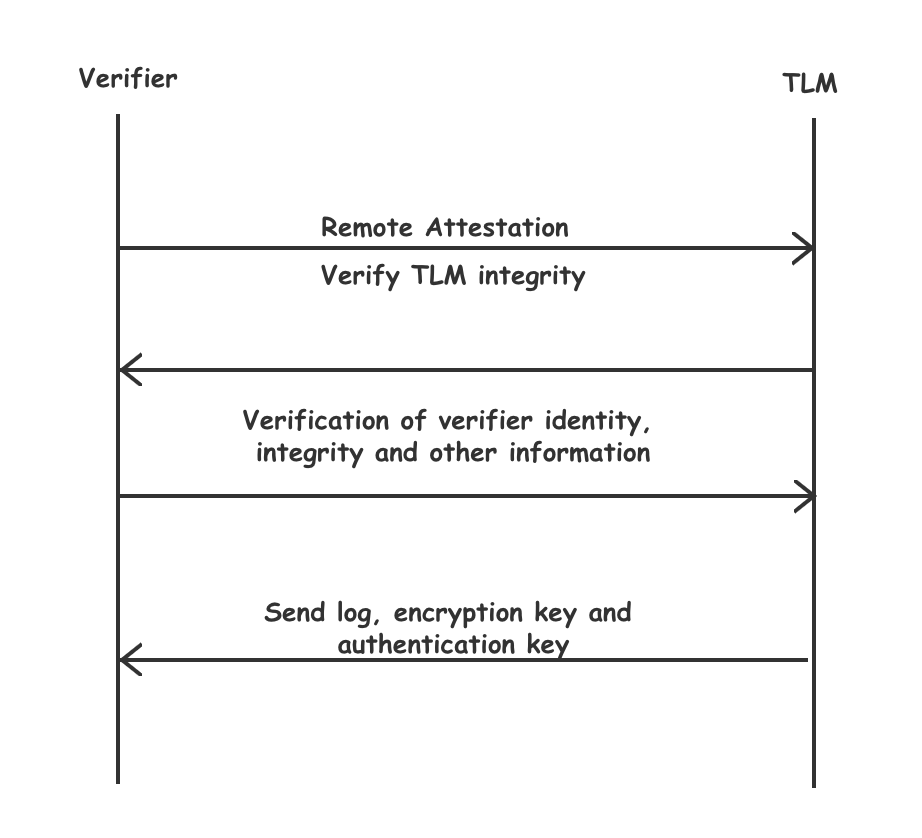
\includegraphics[width=0.8\textwidth]{Fig7}
    \caption{Verify Log}
\end{figure}

In this way, you can view the system log and analyze whether the server obtains, for example, to allow users to obtain the latest information of contacts, such as online status and real-time personal information. 
At the same time eliminate the dependence on trusted servers, and ensure the confidentiality and integrity of log data.

As discussed in this section, through the E2EE protocol plus log security audit, a good message service framework can be implemented. \\

However, in order to minimize the damage caused by attacking the server, you can add data timing destruction, client data encryption storage, you can actively delete server data, etc.


\question{4}{Conclusion}
Encrypt in the instant messaging protocol to ensure that no third party can eavesdrop on the data except the sender and the receiver. The only safe way to achieve this is E2EE (End-to-End Encryption), which is mainly asymmetric 
Way to achieve risk-free encrypted data transmission, even the transmission server can not know the content of the transmission.\\

From the issue1 use of the signal protocol to realize the design of group chat encryption, Signal Protocol is a truly end-to-end encrypted communication protocol that provides forward and backward security of messages and is one of the most secure encryption protocols. 
But at the same time, if there are too many group members, the amount of encryption and decryption operations is very large, which will affect the sending and receiving speed. At the same time, the key management database will also be very large and the reading efficiency will be reduced. 
Therefore, the group chat uses the signal protocol protocol, the group number should not be too much.\\

From issue2, the use of E2EE plus log security audit message service can also provide a good choice. 
However, the default use of E2EE encryption is the minimum standard for a qualified encrypted communication application.\\

Although E2EE is very powerful, it is not only without using E2EE that there is no worry. E2EE is only the foundation, and achieving excellent messaging services requires many considerations and technical combinations.\\

At the same time, in the implementation of E2EE, different applications have different solutions, and safe code implementation is the prerequisite and guarantee. It is best to use the E2EE protocol that has been recognized and safe after years of development and verification rather than the protocol created by yourself.

\end{document}